\documentclass[conference]{IEEEtran}
\IEEEoverridecommandlockouts
% The preceding line is only needed to identify funding in the first footnote. If that is unneeded, please comment it out.
\usepackage{cite}
\usepackage{amsmath,amssymb,amsfonts}
\usepackage{algorithmic}
\usepackage{graphicx}
\usepackage{textcomp}
\usepackage{subfig}
\usepackage[inline]{enumitem}
\usepackage{float}
\usepackage{draftwatermark}
\usepackage{xcolor}
\def\BibTeX{{\rm B\kern-.05em{\sc i\kern-.025em b}\kern-.08em
    T\kern-.1667em\lower.7ex\hbox{E}\kern-.125emX}}
\begin{document}

\SetWatermarkText{WhalingGuard}
\SetWatermarkScale{0.8}
\SetWatermarkColor[gray]{0.9}

\title{WhalingGuard : Phishing Detection Using Machine Learning}
\author{
  \IEEEauthorblockN{Adithyan M S}
  \IEEEauthorblockA{\textit{Department of CSE} \\
\textit{CEM-Punnapra}\\
Alappuzha, India \\
adithyan2ms@gmail.com\\}
  \and
  \IEEEauthorblockN{Harikrishnan K B}
  \IEEEauthorblockA{\textit{Department of CSE} \\
\textit{CEM-Punnapra}\\
Alappuzha, India \\
baluoger91@gmail.com\\}
  \and
  \IEEEauthorblockN{Aswani N K}
  \IEEEauthorblockA{\textit{Department of CSE} \\
\textit{CEM-Punnapra}\\
Alappuzha, India \\
nkaswaniachu@gmail.com\\}
  \and
  \IEEEauthorblockN{Amal Soman}
  \IEEEauthorblockA{\textit{Department of CSE} \\
\textit{CEM-Punnapra}\\
Alappuzha, India \\
amalsoman04@gmail.com\\}
  \and
  \hspace{0.4cm}
  \IEEEauthorblockN{Krishnapriya V J}
  
  \IEEEauthorblockA{\hspace{0.4cm}\textit{Asst. Professor, Department of IT} \\
  \hspace{0.4cm}
\textit{CEM-Punnapra}\\ \hspace{0.4cm}
Alappuzha, India \\ \hspace{0.4cm}
krishnapriyavj@gmail.com\\}
}


\maketitle

\begin{abstract}
Phishing is a type of cyberattack that aims to steal sensitive information such as usernames, passwords, and credit card details. Phishing attacks have become increasingly sophisticated and prevalent in today's digital world. Thus the development of the phishing detection model is essential to combat the increasing threat of phishing attacks, protect users from fraud and data breaches, and enhance overall cybersecurity in the digital landscape. Several machine learning algorithms have been proposed to detect phishing websites by analyzing various features. In this research paper, we compare several machine learning algorithms to detect phishing websites using a dataset of 545,895 samples which is created by pre-processing and merging two separate datasets. We use 74 features to train and evaluate the algorithms, and we found that Logistic Regression(LR) achieved the highest accuracy of 94.44\% after comparing models. The trained LR model is integrated into our WhalingGuard Web Application for predicting whether the input URL from the user interface is phishing or non-phishing.
\end{abstract}

\begin{IEEEkeywords}
Phishing, Machine Learning, Logistic Regression, 
\end{IEEEkeywords}

\section{Introduction}

\par 
Phishing detection is a crucial aspect of cybersecurity aimed at identifying and preventing phishing attacks. Phishing refers to a malicious practice where cybercriminals impersonate legitimate entities or organizations to deceive individuals into sharing sensitive information such as passwords, financial details, or personal data. These attackers often use email, text messages, or deceptive websites to trick unsuspecting users.
\par Phishing attacks can have severe consequences, including identity theft, financial loss, and compromise of sensitive data. To combat this threat, various techniques and technologies have been developed to detect and mitigate phishing attempts[1].Phishing detection involves the use of sophisticated algorithms, machine learning models, and behavioral analysis to identify patterns and indicators that differentiate legitimate communications from phishing attempts. 36\% of all data breaches involved phishing according to Verizon’s 2022 report[2]. It was estimated that by 2022 a ransomware or phishing attack will occur every 11 seconds.

\par Website phishing, also known as phishing websites or fake websites, refers to the creation of fraudulent websites that mimic legitimate websites to deceive users into revealing sensitive information or performing malicious actions[3]. These phishing websites are designed to look and feel like the real ones, often imitating the branding, layout, and functionality of trusted organizations, businesses, or online services. The Phishing statistics suggests that compare to malware sites, phishing sites are 75\% higher in presence. It was identified that 61\% of subjects in a study conducted could not differentiate between a real and a fake Amazon login page[4].So a process/system for identifying and mitigating phishing attacks that occur through fraudulent websites should be implemented Website, which is termed as website phishing detection.

\par In this context, we suggest a phishing detection model
based on machine learning that can detect whether a website URL
relates to phishing or not. \textbullet{} We have compared 15 different
machine learning algorithms for the development of this phishing detection model. \textbullet{} We extracted 74 different features from about 5.5 lakh URLs. And these features where used for training and testing the model. \textbullet{} For comparing the models, we use python-pycaret library and found that Logistic Regression provides better accuracy than any other machine learning algorithms, thus the model is evaluated using Logistic Regression Algorithm. \textbullet{} We have developed a web application that accepts input URLs from the user to predict whether it is phishing or legitimate based on the evaluated model.

\section{RELATED WORKS}
\hspace{.2cm}Sufficiency of Ensemble Machine Learning Methods for Phishing Websites Detection [5] 2021 : Phishing instances are usually derived from PhishTank
Other legitimate instances are from Alexa, DMOZ, and Common Crawl.
Features used in phishing detection are usually extracted from URLs (protocol, domain, path, parameters) This feature selection framework achieves a remarkable 87.6\% reduction in feature quantity with suffering from only a 0.1\% deterioration in detecting accuracy, making it possible for up-date training and real-time detecting in a production environment. Web Phishing Detection Using Machine Learning 
[6] 2022 : Suggest a literacy-based strategy to categorize Web sites into three
categories: benign, spam, and malicious. Our technology merely
examines the Uniform Resource Locator (URL) itself, not the
content of Web pages. As a result, it removes run-time stillness
and the risk of drug users being exposed to cyber surfer-based
vulnerabilities. When compared to a blacklisting service, our
approach performs better on generality and content since it uses
learning techniques. Comparison of Classification Algorithms for Detection of Phishing Websites
[7] 2020 : Compare classic supervised machine learning algorithms on all publicly available phishing datasets with predefined features and to distinguish the best performing algorithm for solving the problem of phishing websites detection, regardless of a specific dataset design.
 
\hspace{.2cm} Phishing Detection using Random Forest, SVM and Neural Network with Backpropagation
[8] 2020 : The paper explains the improved Random Forest classification method, SVM classification algorithm and Neural Network with backpropagation classification methods which have been implemented with accuracies of 97.369\%, 97.451\% and 97.259\% respectively. PhishHaven—An Efficient Real-Time AI Phishing URLs Detection System [9] 2020 : Design a PhishHaven which detects and classifies a URL using three subcomponents.
First subcomponent, URL Hit 
The second subcomponent is Features Extractor.
The third subcomponent is Modelics.In this new paradigm executes ensemble-based machine learning models in parallel using multi-threading technique, and results in real-time detection by significant speed-up in the classification process. Characteristics of Understanding URLs and Domain Names Features: The Detection of Phishing Websites With Machine Learning Methods [10] 2022 : In this study, used a dataset with 32,928 data in which 12,134 data without phishing websites, and 20,614 data with phishing websites to be labeled according to eleven predetermined features.  Experimental results show that phishing websites can be detected with as much as 98.90\% accuracy with our proposed method. As a result, it has been demonstrated that RF descriptors with SVM representation can be utilized to accurately mark phishing web pages. In addition, characteristic updates can be followed with a continuously updated source.

\hspace{.2cm} Detection of Phishing Websites using Machine Learning [11] 2021 : Collect unstructured data of URLs from Phishtank website, Kaggle website and Alexa website, etc.
Train the three unique classifiers and analyse their presentation based on exactness two classifiers utilized are Decision Tree and Random Forest algorithm. Each classifier is trained using training set and testing set is used to evaluate performance of classifiers.
Performance of classifiers has been evaluated by calculating classifiers accuracy score.  Eth-PSD: A Machine Learning-Based Phishing Scam Detection Approach in Ethereum
[12] 2021 :  Detect phishing scam-related transactions using a novel machine learning-based approach. Eth-PSD tackles some of the limitations in the existing works, such as the use of imbalanced datasets, complex feature engineering, and lower detection accuracy. Proposed Eth-PSD to detect the phishing scam in Ethereum. Started with derived requirements based on the limitations of related works and other effective IDSs from previous related works.





\section{PROPOSED WORK}

\par In this section, we describe the phishing detection
framework which consists of two major parts as shown in Fig:1. The first part is the Training Phase and the second part is the Detection Phase. In
the first phase, datasets containing URLs are prepared for the machine learning algorithm and model is evaluated. In the second phase, an input URL is received from the user and based on the evaluated model, the URL is classified into phishing or legitimate.

\begin{figure}[H]
\centerline{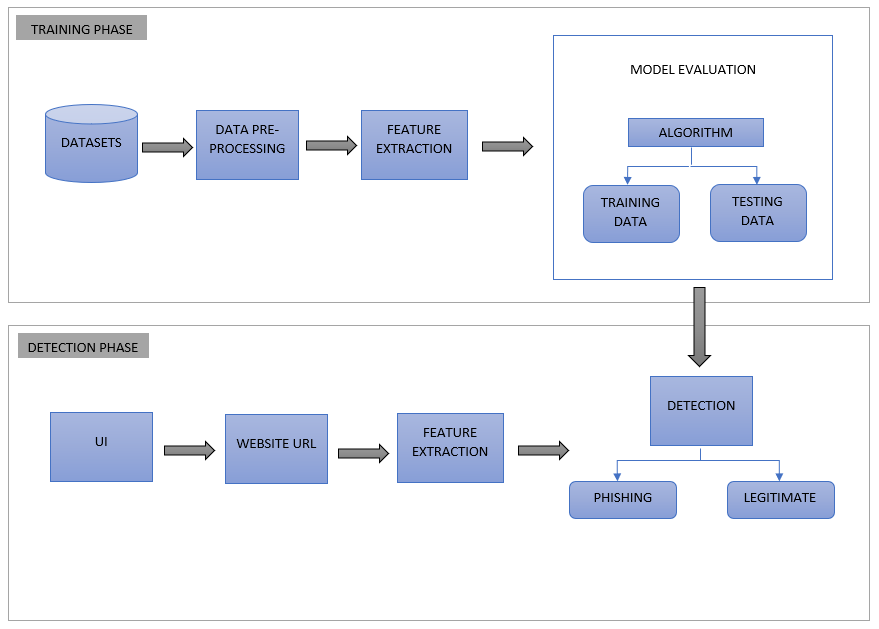
\includegraphics[scale=0.3]{newModel.png}}
\caption{System Architecture}
\label{fig}
\end{figure}
\subsection{TRAINING PHASE}

\subsection*{I. {\footnotesize DATASET}}
The dataset is created by merging two different datasets to improve the efficiency of prediction.
\begin{enumerate}
    \item Dataset-I
\par This dataset is collected from phishtank.com which contains 96,020 data with 50\% phishing and 50\% of legitimate URLs. This dataset contains columns - domain and label,where domain represents the URLs and label denotes whether the URL is phishing or legitimate by representing 1 and 0 respectively.
    
    \item Dataset-II
\par This dataset is collected from Kaggle.com which contains 450,176 data, having URL, label and result as columns.
\end{enumerate}
\begin{figure}[H]
\centerline{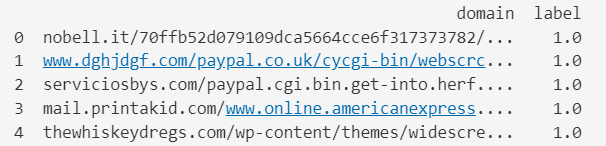
\includegraphics[scale=0.58]{dataset1.png}}
\caption{Dataset-I from phishtank.com}
\label{fig}
\end{figure}
\begin{figure}[H]
\centerline{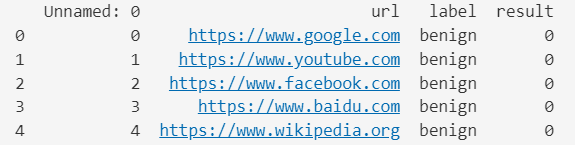
\includegraphics[scale=0.6]{dataset2.png}}
\caption{Dataset-II from kaggle.com}
\label{fig}
\end{figure}


\subsection*{II. {\footnotesize DATA PREPROCESSING}}
Data pre-processing is an essential step in preparing raw data for analysis and machine learning tasks. It involves transforming and cleaning the data to ensure its quality, consistency, and suitability for further analysis.
We obtained two separate datasets from different sources and merged them to create a larger dataset for training and testing our machine learning models.

\par In the Dataset-I (url and label as columns), we found 92 URLs without any corresponding label values i.e, having null values. and these rows were dropped from this datasets. We only need the URLs and there corresponding label values(1 0r 2 representing phishing or legitimate) as the input datas, the Dataset-II contains unwanted columns so they are also dropped. Next we will be merging our 2 datasets , for that we will be considering the Datatypes and names of the columns to avoid damage of the resultant dataset after merging.Merging DataFrames with different data types for the same column name might lead to inconsistencies and unexpected behavior and merging DataFrames having different column names produce splitting of the values. So they both are handled before merging. After Merging we obtained a dataset having 546,104 datas and saved in a new csv file.
\par After merging there are chances of having duplicate data inside the resultant dataset. There were 194 Duplicate URLs in our resultant dataset. And these were dropped. Fig 4. shows the 
Bar-Graph Classification of Phishing and Legitimate URLs inside the new dataset:

\begin{figure}[H] 
  \centering
  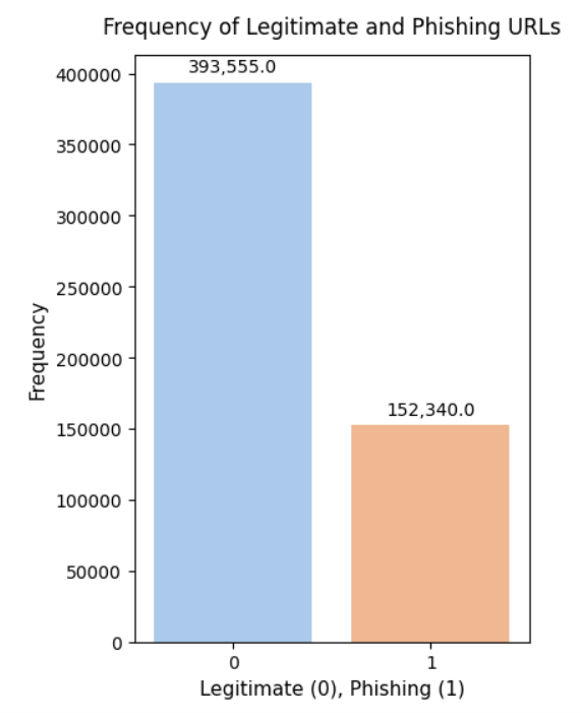
\includegraphics[scale=0.4]{total frequency.png} 
  \caption{Bar-Graph Classification of Phishing and Legitimate data.}
  \label{fig}
\end{figure}
\subsection*{III. {\footnotesize FEATURE EXTRACTION}}
\par Feature extraction is a technique used to reduce the dimensionalities of data by transforming the raw input into a set of derived features that capture the essential information. It aims to highlight the most relevant aspects of the data and discard irrelevant or redundant information. 
\par In our project, the features are generally classified into two:
\begin{enumerate}
  \item Lexical Features
  \item Numerical Features
\end{enumerate}
\subsection*{1) Lexical Features}
\par Lexical features in URL feature extraction involve analyzing the textual components and patterns within a URL. These features capture characteristics related to the structure, keywords, symbols, and other textual elements of a URL.
\begin{itemize}
  \item getEntropy :-{ It is known that DGA(Domain Generation Algorithm) domains have a greater level of disorderliness in their alphabetic distribution. Legitimate domains tend to have well-defined names that speak to a brand or a product so tend to be less disorganized. Thus, measuring the entropy of URL strings tells us which domain names are ‘not-so-real.}
  \item hasLogin :-{Check if the URL contains specific keyword "login," .We can capture the fact that certain ‘red flag’ keywords appear in a URL string. These keywords may relate to keywords attackers use when trying to spoof a legitimate page or keywords that relate to popular nomenclature of security settings on a website that a hacker will try to manipulate.So,If the URL string contains “login” keyword, the value assigned to this feature is 1 (phishing) or else 0 (legitimate).}
  \item Redirection :-{ Phishing attackers often employ redirection techniques to hide the true destination of a malicious URL. By redirecting users through multiple URLs or using URL shorteners, they can make it more difficult for users and security systems to identify the final destination. Checks the presence of "//" in the URL. The existence of “//” within the URL path means that the user will be redirected to another website.(avoiding the "//" after the http/https)}
  \item lenClassify :-{Computes the length of the URL. Phishers can use long URL to hide the doubtful part in the address bar. In this project, if the length of the URL is greater than or equal 54 characters then the URL classified as phishing otherwise legitimate. If the length of URL >= 54 , the value assigned to this feature is 1 (phishing) or else 0 (legitimate).}
  \item haveAtSign :-{Checks for the presence of '@' symbol in the URL. Using “@” symbol in the URL leads the browser to ignore everything preceding the “@” symbol and the real address often follows the “@” symbol.And also used to mimic or spoof well-known websites or services. If the URL has '@' symbol, the value assigned to this feature is 1 (phishing) or else 0 (legitimate).}
  \item getDepth :-{The depth of a URL refers to the number of hierarchical levels or directories in the URL's path. It represents how nested a specific resource is within a website's directory structure. This feature calculates the number of sub pages in the given URL based on the '/'.}
  \item tinyURL :-{URL shortening is a method in which a URL are shortened and can still lead to the required webpage. And this is accomplished by most of the phishing websites.If the URL is using Shortening Services, the value assigned to this feature is 1 (phishing) or else 0 (legitimate).}
  \item isDomainIp :-{Some Phishing URLs represents the domain name by IP address instead of hostname. Checks for the presence of IP address in the URL. URLs may have IP address instead of domain name. If an IP address is used as an alternative of the domain name in the URL, we can be sure that someone is trying to steal personal information with this URL.If the domain part of URL has IP address, the value assigned to this feature is 1 (phishing) or else 0 (legitimate).}
  \item prefixSuffix :-{Checking the presence of '-' in the domain part of URL. The dash symbol is rarely used in legitimate URLs. Phishers tend to add prefixes or suffixes separated by (-) to the domain name so that users feel that they are dealing with a legitimate webpage.If the URL has '-' symbol in the domain part of the URL, the value assigned to this feature is 1 (phishing) or else 0 (legitimate).}
\end{itemize}
\subsection*{2) Numerical Features}
\par Numerical value-based features are features that represent quantitative or continuous values. These features can take on a wide rang
e of numeric values and are often used in various machine learning algorithms and statistical analyses. 

% \begin{figure}[htbp]
% \centerline{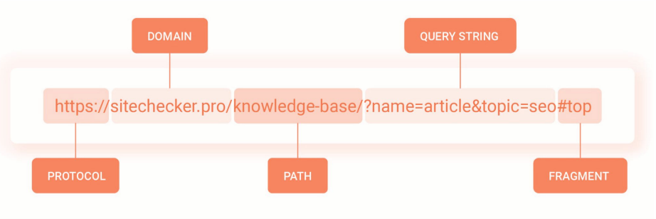
\includegraphics[scale=0.25]{urlfeat.png}}
% \caption{Basic structure of a URL}
% \label{fig}
% \end{figure}
\par Features of a URL are basically classified into - protocol, domain, path, query, fragment. The length of this each features and the count of the different special characters in that specific feature are extracted. The special characters like  ‘.’ ‘-’ ‘/’ ‘?’ ‘=’ ‘@’ ‘\&’ ‘!’ ‘\ ’ ‘\textasciitilde' ‘,’ ‘+’ ‘*’ ‘\#’ ‘\$’ ‘\%’ .
\par These features are : \begin{enumerate*}[label=\textbullet]
\item url\_length,\item qty\_dot\_url,\item qty\_hyphen\_url,\item qty\_slash\_url,\item qty\_questionmark\_url,\item qty\_equal\_url,\item qty\_at\_url,\item qty\_and\_url,\item qty\_exclamation\_url,\item qty\_space\_url,\item qty\_tilde\_url,\item qty\_comma\_url,\item qty\_plus\_url,\item qty\_asterisk\_url,\item qty\_hashtag\_url,\item qty\_dollar\_url,\item qty\_percent\_url,\item domain\_length,\item qty\_dot\_domain,\item qty\_hyphen\_domain,\item path\_length,\item qty\_dot\_path,\item qty\_hyphen\_path,\item qty\_slash\_path,\item qty\_equal\_path\item qty\_at\_path,\item qty\_and\_path,\item qty\_exclamation\_path,\item qty\_space\_path,\item qty\_tilde\_path,\item qty\_comma\_path,\item qty\_plus\_path,\item qty\_asterisk\_path,\item qty\_dollar\_path,\item qty\_percent\_path,\item query\_length,\item qty\_dot\_query,\item qty\_hyphen\_query,\item qty\_slash\_query,\item qty\_questionmark\_query,\item qty\_equal\_query,\item qty\_at\_query,\item qty\_and\_query,\item qty\_exclamation\_query,\item qty\_space\_query,\item qty\_tilde\_query,\item qty\_comma\_query,\item qty\_plus\_query,\item qty\_asterisk\_query,\item qty\_dollar\_query,\item qty\_percent\_query,\item fragment\_length,\item qty\_dot\_fragment,\item qty\_hyphen\_fragment,\item qty\_slash\_fragment,\item qty\_questionmark\_fragment,\item qty\_equal\_fragment,\item qty\_and\_fragment,\item qty\_exclamation\_fragment,\item qty\_space\_fragment,\item qty\_comma\_fragment,\item qty\_asterisk\_fragment,\item qty\_hashtag\_fragment,\item qty\_dollar\_fragment,\item qty\_percent\_fragment
\end{enumerate*}.
\par Finally, a total of 74 features are extracted in this project. After extracting both the Lexical and Numerical Features, they are saved to a new csv file for the Model Evaluation.


\subsection*{IV. {\footnotesize MODEL COMPARISON}}
\subsubsection*{Pycaret}
\par PyCaret is a Python library that provides an easy-to-use interface for training and comparing multiple machine learning models. It offers a variety of functions and tools to streamline the model development process and make it efficient. We use this library to compare the different machine learning models by using the extracted features and it will returns a table of model performance metrics sorted by  specified evaluation metrics - accuracy, AUC, recall, precision, F1, Kappa and MCC.

\par 15 different algorithms were compared and Logistic Regression(94.45\%) gave more accuracy among them. Thus, Logistic Regression model is used for testing and training the features.  
\subsubsection*{Logistic Regression}\\
\par Logistic regression is a statistical modeling technique used for binary classification problems, where the goal is to predict the probability of an event or the likelihood of an outcome falling into one of two classes. Despite its name, logistic regression is a classification algorithm rather than a regression algorithm. It is based on the assumption that the relationship between the input variables (also known as independent or predictor variables) and the log-odds of the binary outcome (dependent or response variable) can be approximated by a linear relationship.
\begin{figure}[H]
\centerline{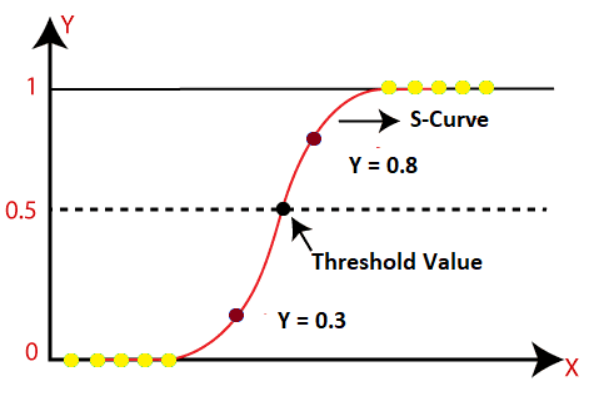
\includegraphics[scale=0.4]{LRgraph.png}}
\caption{Logistic Regression}
\label{fig}
\end{figure}
\par The logistic function, also called the sigmoid function, is used to map the linear combination of input variables to a range between 0 and 1, representing the probability of belonging to the positive class. The logistic function is given by:
\[
p(x) = \frac{1}{1 + e^{-z}}
\]


where p(x) is the predicted probability, x is the input variables, and z is the linear combination of the input variables.

\subsection*{V. {\footnotesize MODEL EVALUATION}}
\par Model evaluation is a crucial step in machine learning to assess the performance and effectiveness of a trained model. It involves quantitatively measuring how well the model generalizes to new, unseen data and how accurately it predicts the target variable.Based on the model comparison, we evaluated the logistic regression(LR) model in this project.

\par Evaluating the LR model includes the following steps:
\begin{itemize}
\item Splitting the dataset: Dividing dataset into training and testing sets, ensuring that both sets have a representative distribution of the target variable.
\item Training the LR model: Fitting the logistic regression model to the training data using a suitable library such as scikit-learn.
\item Make predictions: Use the trained model to predict the target variable for the test dataset.
\item Calculating evaluation metrics: Comparing the predicted values with the actual values from the test dataset and calculating the evaluation metrics such as accuracy, precision, recall, F1-score, AUC-ROC, and confusion matrix. Libraries like scikit-learn provide functions to calculate these metrics.
\end{itemize}


\subsection*{VI. {\footnotesize MODEL IMPLEMENTATION}}
\par This phase involves deploying and integrating the trained machine learning model into a production environment where it can be used to make predictions on new, unseen data.This includes the following processes:
\begin{itemize}
\item Exporting the Model: Saving the trained model in a serialized format that can be easily loaded and used for predictions. We will be using python pickle module for exporting the trained LR model, which is a built-in module that provides a way to serialize and deserialize Python objects.
\item Model Integration: Integrating the model into the target application which is the WhalingGuard Web Application where it will be used for predictions by API call.
\item Model Loading: Loading the serialized model into the implementation environment, making it ready for use. Again the pickle module is used to deserialize the model.
\item Input Data Feeding: Providing the new data, which is the URL to the model for prediction. This is done by passing the input data through an API call from the WhalingGuard User-Interface.
\item Feature Extraction: Extract the 74 different features from the input URL that where extracted during training phase. And saving that features to a new file for predicting.
\item Prediction Generation: Utilize the loaded model to generate predictions on the extracted features. Fitting the loaded model to the extracted features.  
\item Output Delivery: The prediction result is then passed to the API and the API then sends the results as a response to the frontend. The prediction results is also saved in csv file in the server, continuously for each API calls.Then, at the user interface, the users can view the results whether the entered URL is phishing or non-phishing.
\end{itemize}
\\
\subsection{DETECTION PHASE}
\subsection*{I. {\footnotesize USER INTERFACE}}
\par  A web application with a user interface that interacts with an API is developed as part of this project for getting the URL from the user and displaying the corresponding detection result, based on our model.This Web Application is set up with two separate projects: one for the frontend (React) and one for the backend (Node.js API). For the FrontEnd, we used Reactjs framework and has made a HTTP request to the backend API endpoints to fetch and update data. The Backend API is developed using Nodejs and appropriate code are written for handling the request, processing the data, and sending responses back to the frontend.
\subsection*{II. {\footnotesize DETECTION}}
\par The input URL from the user interface is detected either as Phishing or Non-Phishing.
\begin{itemize}
    \item Phishing: Type of URLs that are specifically designed to deceive users by impersonating legitimate websites or services.
    \item Non-Phishing Type of URLs that are the genuine URLs of legitimate websites or services.
\end{itemize}


\section{RESULTS AND DISCUSSION}

\subsection{Feature Analysis}
\subsubsection*{Boxplot Graph}
\par The boxplot graph is a useful visualization for displaying the distribution of a numerical feature or variable. It is employed to explore and understand the distribution of feature values during the analysis of the dataset.By creating the boxplot graph, we could gain insights into the distribution of feature values, including measures of central tendency, dispersion, mean and identification of outliers. Visualization of some features are shown below:

\begin{figure}[H]
  \centering
  \subfloat[getEntropy]{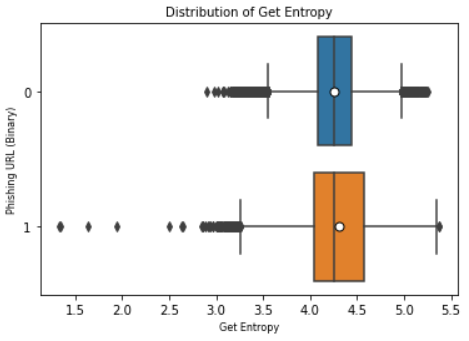
\includegraphics[width=0.2\textwidth]{getEntropy.png}\label{fig:figure1}}
  \hfill
  \subfloat[hasLogin]{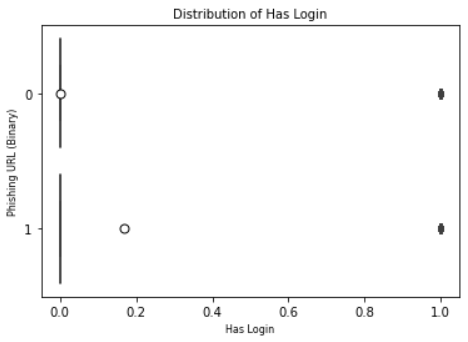
\includegraphics[width=0.2\textwidth]{hasLogin.png}\label{fig:figure2}}
  \label{fig:bothfigures}
\end{figure}

\begin{figure}[H]
  \centering
  \subfloat[getDepth]{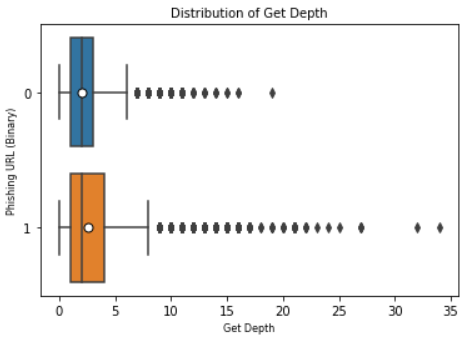
\includegraphics[width=0.2\textwidth]{getDepth.png}\label{fig:figure1}}
  \hfill
  \subfloat[urlLength]{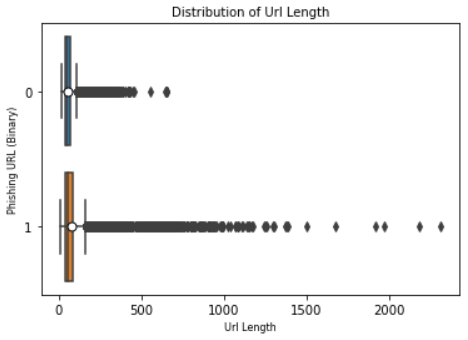
\includegraphics[width=0.2\textwidth]{urlLength.png}\label{fig:figure2}}
  \caption{Visualization of URL features}
  \label{fig:bothfigures}
\end{figure}

\par Visually, we see that legitimate URLs have higher entropy and are generally longer than phishing URLs.Similarly, we can capture the fact that ‘red flag’ keywords appear in a URL string which is the keyword ‘login’, is more seen in the phishing URLs. The depth of the URL i.e, number of hierarchical levels or directories in the URL’s path for phishing URLs is seen greater than the legitimate ones. It is also seen that the phishing URLs have higher URL length than the legitimate URLs.
\subsection{Pycaret Analysis}

\begin{figure}[H]
\centerline{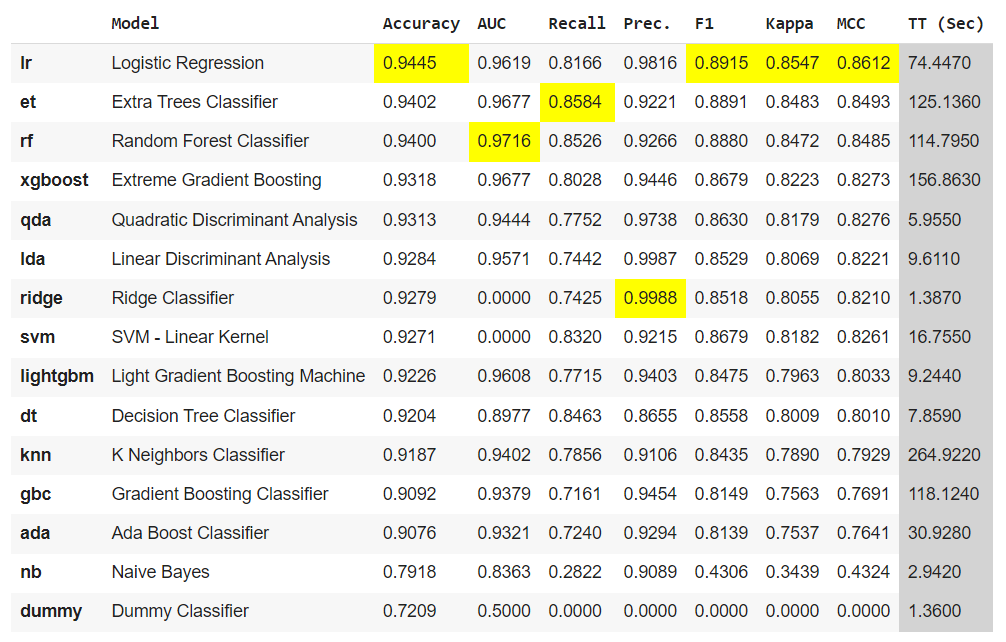
\includegraphics[scale=0.35]{pycaretCheck.png}}
\caption{Pycaret Comparison}
\label{fig}
\end{figure}

\par When using PyCaret for model comparison, the results obtained can provide valuable insights into the performance of different machine learning algorithms on the given dataset.The comparison results obtained using PyCaret can guide in selecting the most suitable machine learning model(s) for this project, taking into account performance metrics, statistical significance, feature importance, and other relevant factors. Fig:8 shows the comparison result.
\subsection{Model Analysis}
\begin{figure}[H]
\centerline{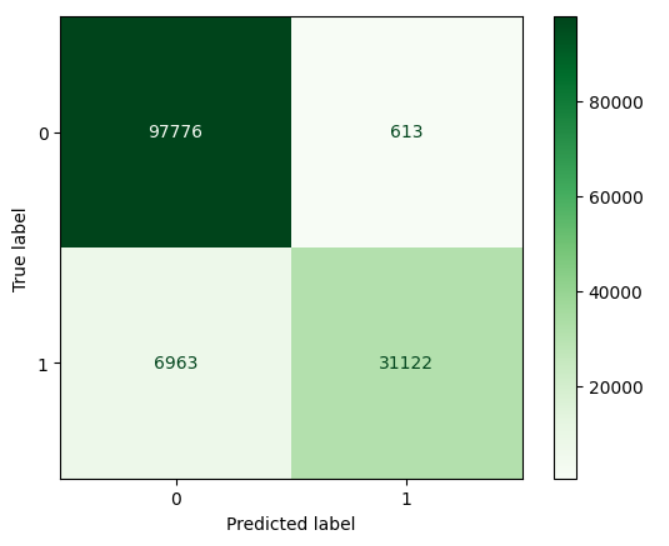
\includegraphics[scale=0.5]{greenCN.png}}
\caption{Confusion Matrix}
\label{fig}
\end{figure}


\par A confusion matrix is a table that is used to evaluate the performance of a classification model. It shows the number of true positives (TP), true negatives (TN), false positives (FP), and false negatives (FN) by comparing the predicted labels with the true labels of a dataset. The confusion matrix provides a more detailed understanding of the model's performance beyond simple accuracy. From the confusion matrix, some of the evaluation metrics calculated in our project are shown in fig:10
\begin{figure}[H]
\centerline{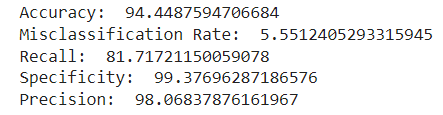
\includegraphics[scale=0.75]{CMvalues.png}}
\caption{Evaluation metrics}
\label{fig}
\end{figure}
% \par Based on the Logistic Regression Model, it has assigned feature importance score to each extracted features. It helps to provide insights into which features have the most influence on the model's predictions. Fig:11 shows the importance of some of the features in our project in the descending order.
% \begin{figure}[H]
% \centerline{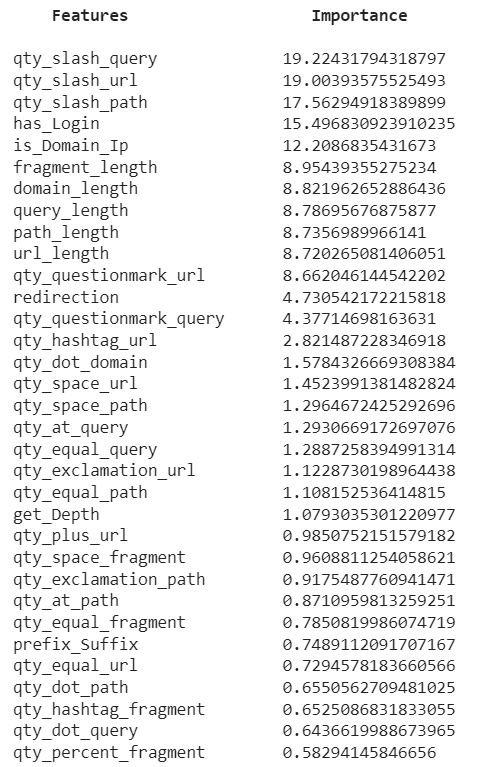
\includegraphics[scale=0.55]{featImp1.png}}
% \caption{Features and their importances}
% \label{fig}
% \end{figure}

\subsection{Web Application}
\par We have developed a web application where the users can input URLs to check if it is phishing or non-phishing.The UI of the application is developed using Reactjs and the API setup for the application is implemented using Nodejs. Fig:12 shows the User Interface of the WhalingGuard web application.
\begin{figure}[H]
\centerline{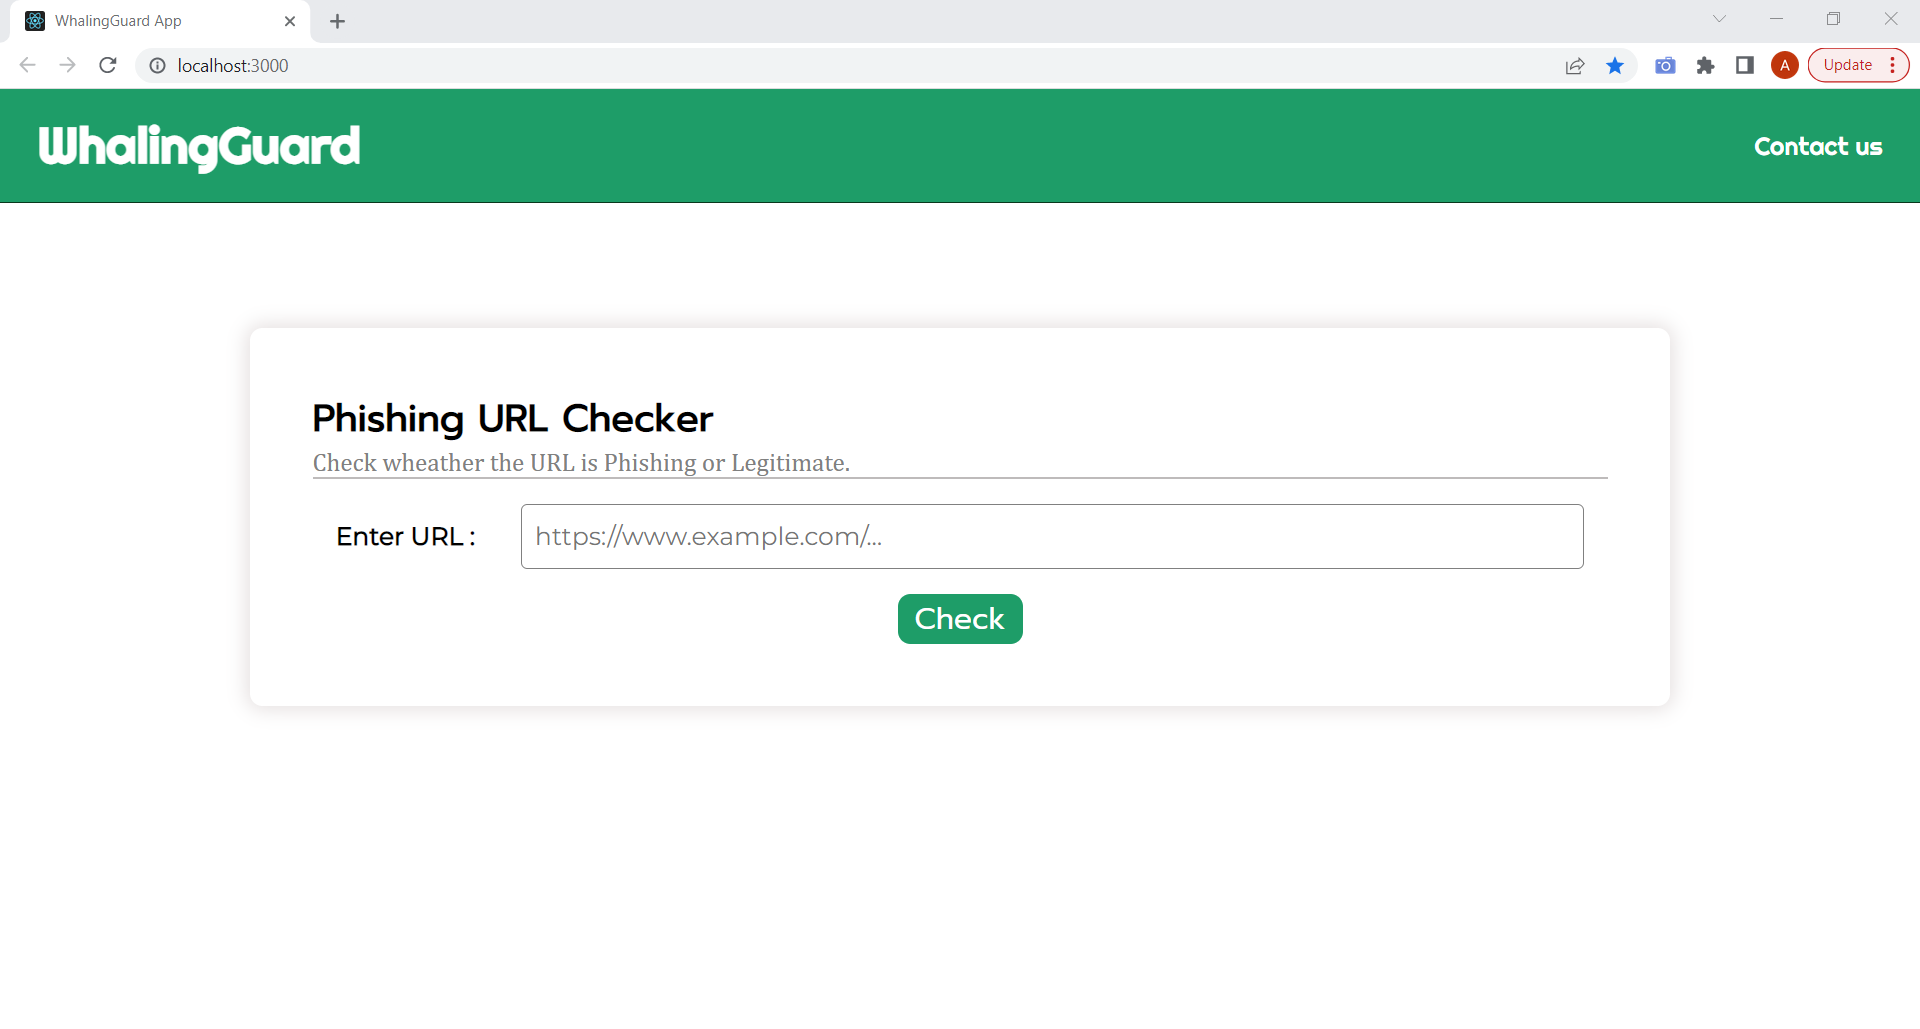
\includegraphics[scale=0.2]{ui.png}}
\caption{User Interface}
\label{fig}
\end{figure}
\par The URL entered by the user is received by the server and it is predicted by the evaluated LR model.Based on the prediction, the summary of the result is shown as output in the user-interface. The following figures shows the 2 different output produced.
\begin{figure}[H]
\centerline{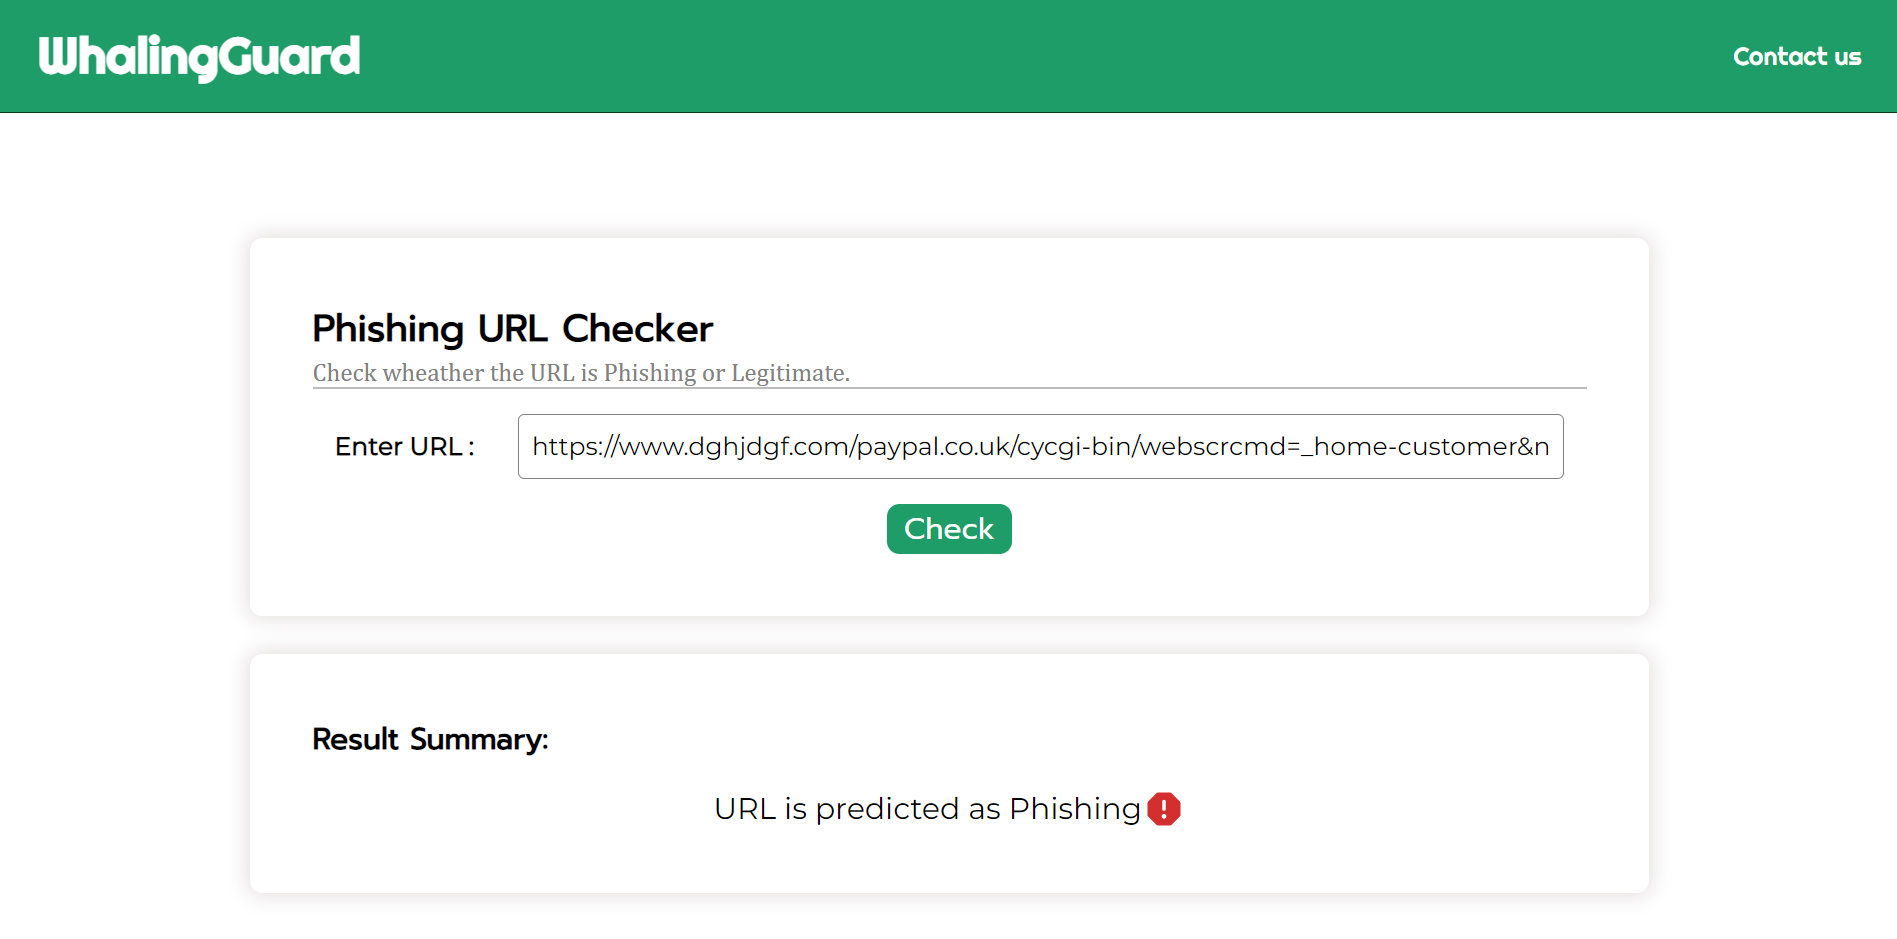
\includegraphics[scale=0.2]{uiP.png}}
\end{figure}
\begin{figure}[H]
\centerline{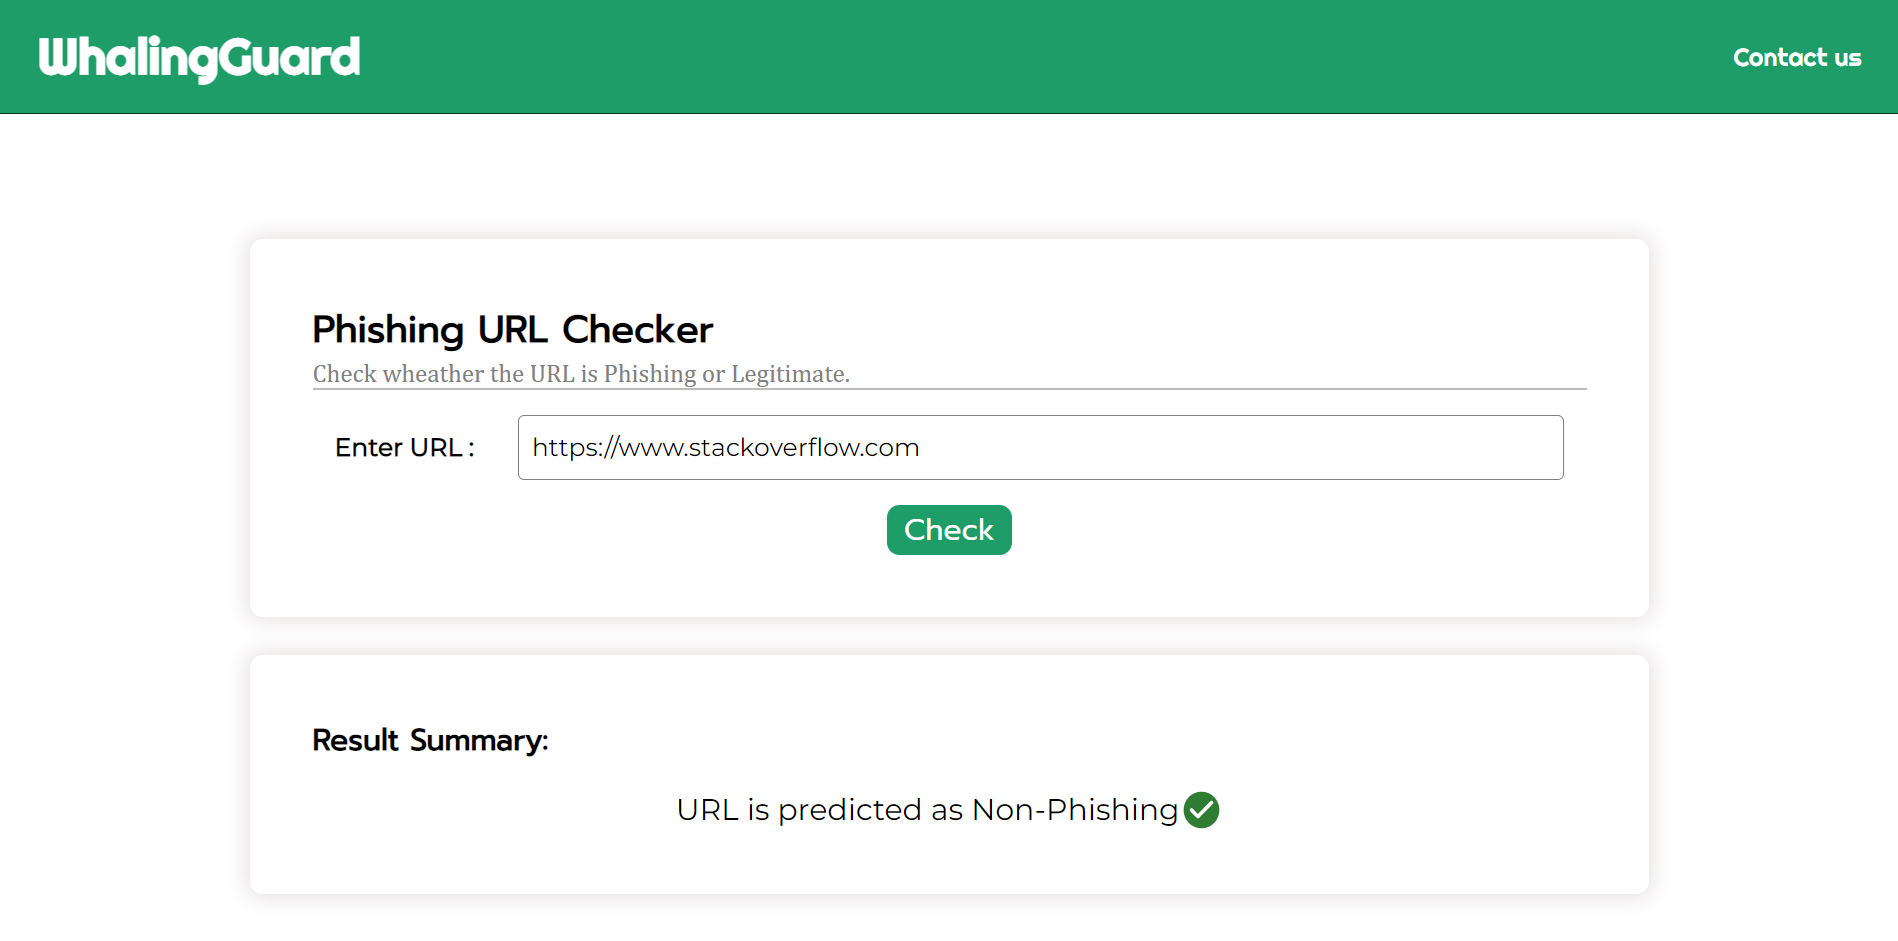
\includegraphics[scale=0.2]{uiN.png}}
\caption{Prediction Results}
\label{fig}
\end{figure}

\section{CONCLUSION}
\par In particular, phishing has become more common and
has begun to raise significant issues. There needs to design phishing 
 detection method to affectively detect if the website is phishing or non-phishing. Considering the significance of phishing detection,
in this study, we extracted 74 different features from the website URL. After comparing different machine learning algorithms, we found that Logistic Regression gives higher accuracy. So we used Logistic Regression model for phishing prediction. In future we are planning to design a
framework for identifying and preventing phishing attacks that are delivered through email messages.


\begin{thebibliography}{00}
\bibitem{b1}Michael A. Ivanov,  Bogdana V. Kliuchnikova,  Ilya V. Chugunkov,  Anna M. Plaksina, ``Phishing Attacks and Protection Against Them,'' 2021.
\bibitem{b2}Michael A. Ivanov,  Bogdana V. Kliuchnikova,  Ilya V. Chugunkov,  Anna M. Plaksina
 , ``Survey on Detection and Prevention of Phishing Websites using Machine Learning,'' 2021.
\bibitem{b3}Hossein Abroshan, Jan Devos, Geert Poels, Eric Laermans
 , ``Phishing Happens Beyond Technology: The Effects of Human Behaviors and Demographics on Each Step of a Phishing Process,'' 2021.
\bibitem{b4} M. D. Bhagwat, P. H. Patil, T. S. Vishawanath, ``A Methodical Overview on Detection, Identification and Proactive Prevention of Phishing Websites
,'' 2021.
\bibitem{b5} Yi Wei, Yuji Sekiya
, ``Sufficiency of Ensemble Machine Learning Methods for Phishing Websites Detection,'' 2021.
\bibitem{b6} N Kumaran, Purandhar
Sri Sai, Lokesh Manikanta.
, ``Web Phishing Detection Using Machine Learning,'' 2022.
\bibitem{b7} Paulius Vaitkevicius, ``Comparison of Classification Algorithms for Detection of Phishing Websites,'' 2020.
\bibitem{b8} Sindhu, Sunil Parameshwar Patil, Arya Sreevalsan, Faiz Rahman, ``Phishing Detection using Random Forest, SVM and Neural Network with Backpropagation,'' 2020.
\bibitem{b9}Maria Sameen, Kyunghyun Han, Seong Oun Hwang , ``PhishHaven—An Efficient Real-Time AI Phishing URLs Detection System 
,'' 2020.
\bibitem{b10} Ilker Kara, Murathan Ok, Ahmet Ozaday, ``Characteristics of Understanding URLs and Domain Names Features: The Detection of Phishing Websites With Machine Learning Methods,'' 2022.
\bibitem{b11} Atharva Deshpande, Omkar Pedamkar, Nachiket Chaudhary , ``Detection of Phishing Websites using Machine Learning,'' 2021.
\bibitem{b12} Arkan Hammoodi Hasan Kabla, Mohammed Anbar, Selvakumar Manickam, Shankar Karupayah, ``Eth-PSD: A Machine Learning-Based Phishing Scam Detection Approach in Ethereum,'' 2021.
\end{thebibliography}
\end{document}
